\documentclass{article}
\usepackage[utf8]{inputenc}
\usepackage{amsmath}
\usepackage{amssymb}
\usepackage{algpseudocode}
\usepackage[a4paper, total={6in, 8in}]{geometry}
\usepackage{graphicx}
\usepackage{multirow}
\usepackage{algorithmicx}
\graphicspath{ {images/} }

\title{Práctica 1 - Aprendizaje Automático}
\author{Luis Miguel Guirado Bautista - Universidad de Granada}
\date{3 de abril de 2022}

\algdef{SE}[DOWHILE]{Do}{doWhile}{\algorithmicdo}[1]{\algorithmicwhile\ #1}%

\renewcommand*\contentsname{Índice}
\renewcommand{\figurename}{Figura}
\renewcommand{\partname}{Ejercicio}

\begin{document}

    \begin{titlepage}
        \maketitle
    \end{titlepage}

    \pagebreak

    \tableofcontents

    \pagebreak 

    \part{Búsqueda iterativa de óptimos}
    \section{Algoritmo de gradiente descendente}
    \raggedright
    El algoritmo de gradiente descendente tiene como objetivo \textbf{optimizar una función} moviendo
    un punto inicial $w_0$ a un óptimo local mediante un vector
    de forma \textbf{iterativa}. El vector encargado de mover nuestro punto $w_j$ depende de la derivada de la
    función a optimizar. Entonces \textbf{si nuestra función no es derivable, entonces el algoritmo no es aplicable}. \par
    En caso de tener más variables, dependerá de las derivadas parciales de cada una de las variables,
    de modo que el punto se moverá en el eje de la variable $j$ según su derivada parcial. \par
    \vspace*{0.2in}
    La actualización del punto $w$ viene dada por la siguiente expresión, siendo $\eta \in \left[0,1\right]$ la \emph{tasa de aprendizaje}
    de nuestro algoritmo y $f$ la función a optimizar
    \begin{equation*}
        w := w - \eta \frac{\partial f}{\partial w}
    \end{equation*}
    El algoritmo se detendrá y devolverá el valor $w$ cuando se haya alcanzado el valor deseado de la función por debajo de un
    valor $\varepsilon$ o cuando el número de iteraciones actual sea mayor que $N$. \par
    Ahora vamos a formalizar la implementación de nuestro algoritmo. \par
    \vspace{0.2in}
    \begin{algorithmic}
        \Function{gradient\_descent}{$w_0$, $\eta$, $f$, $\varepsilon$, $N$}
        %\If{$f$ is not derivable}
        %    \State\Return
        %\EndIf
        \State{$iter \gets 0$}
        \State{$w \gets w_0$}
        \While{$f(w) > \varepsilon$ \textbf{and} $iter \leq N$}
            \State{$iter \gets iter + 1$}
            \State{$w \gets w - \eta \cdot \frac{\partial f}{\partial w}$}
        \EndWhile
        \State{\Return{$(w, iter)$}}
        \EndFunction
    \end{algorithmic}

    \pagebreak
    \section{Ejemplos prácticos}
    \subsection{Función $E$}
    Siendo nuestra función $E(u,v)$:
    \begin{equation*} \label{e}
        E(u,v) \; = \; (uve^{(-u^2-v^2)})^2 \; = \; u^2v^2e^{(-2u^2-2v^2)}
    \end{equation*}
    Podemos ver que $E$ es derivable al ser composición de funciones continuas.
    Por tanto podemos aplicar el algoritmo de gradiente descendente a $E$.
    \linebreak
    La derivada parcial con respecto a $u$ es:
    \begin{equation*} \label{deu}
        \frac{\partial E}{\partial u} = 2uv^2e^{(-2u^2-2v^2)}(1 - 2u^2)
    \end{equation*}
    Y la derivada parcial con respecto a $v$ es:
    \begin{equation*} \label{dev}
        \frac{\partial E}{\partial v} = 2vu^2e^{(-2u^2-2v^2)}(1-2v^2)
    \end{equation*}
    Entonces \textbf{la expresión del gradiente} sería:
    \begin{equation*}
        \frac{\partial E}{\partial w} 
        = \left(\frac{\partial E}{\partial u},\frac{\partial E}{\partial v}\right) 
        = \left(2uv^2e^{(-2u^2-2v^2)}(1 - 2u^2)\;,\;2vu^2e^{(-2u^2-2v^2)}(1-2v^2)\right)
    \end{equation*}
    Ahora, considerando los siguientes parámetros,
    incluyendo nuestra función $E$ y su gradiente $\frac{\partial E}{\partial w}$:
    \begin{center}
        \begin{tabular}{ |c|c|c|c| }
            \hline
            $\eta$ & $N$ & $\varepsilon$ & $w_0$ \\
            \hline
            0.1 & $10^9$ & $10^-8$ & $(0.5,-0.5)$ \\
            \hline
        \end{tabular}
    \end{center}
    Al realizar una ejecución de nuestro algoritmo con estos parámetros, obtenemos los siguientes resultados:
    \begin{itemize}
        \item[]\textbf{Número de iteraciones:} 25117
        \item[]\textbf{Coordenadas alcanzadas:} $w = (0.01,-0.01)$
    \end{itemize}
    \pagebreak
    \begin{figure}[h] \label{fig1}
        \caption{Representación visual de la ejecución del algoritmo sobre $E$}
        \centering
        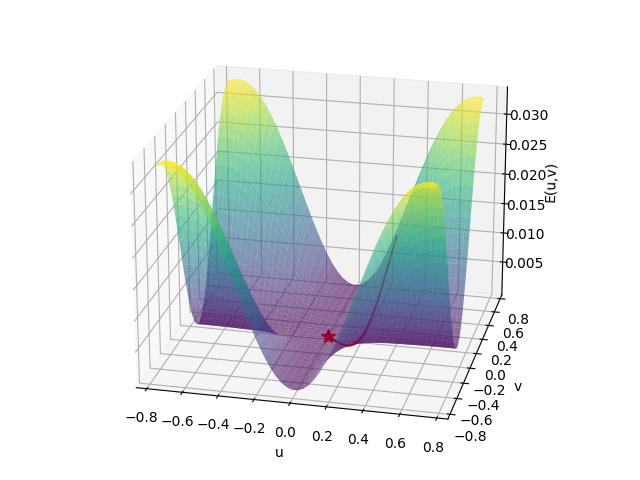
\includegraphics[width=\textwidth]{Figure_1.png}
    \end{figure}
    En la figura 1 podemos ver la función dibujada en un gráfico 3D y el recorrido del algoritmo
    que desemboca en una punto estrellado, que representa el mínimo local alcanzado.
    En este primer ejemplo podemos ver que el algoritmo ha cumplido con su objetivo, ahora veamos un
    segundo ejemplo más complicado.

    \pagebreak

    \subsection{Función $f$}
    Ahora vamos a realizar los mismos pasos con una función $f(x,y):$
    \begin{equation*}
        f(x,y) = x^2 + 2y^2 + 2 \sin{(2 \pi x)}\sin{(\pi y)}
    \end{equation*}
    $f$ es derivable ya que es composición de funciones continuas.

    Calculamos sus derivadas parciales:
    \begin{equation*}
        \frac{\partial f}{\partial x} = 2x + 4 \pi \sin{(\pi y)} \cos{(2 \pi x)}
    \end{equation*}
    \begin{equation*}
        \frac{\partial f}{\partial y} = 4y + 2 \pi \sin{(2 \pi x)} \cos{(\pi y)}
    \end{equation*}
    Por tanto el gradiente de $f$ sería:
    \begin{equation*}
        \frac{\partial f}{\partial w}
        = \left(\frac{\partial f}{\partial x},\frac{\partial f}{\partial y}\right)
        = \big(2x + 4 \pi \sin{(\pi y)} \cos{(2 \pi x)}\;,\;4y + 2 \pi \sin{(2 \pi x)} \cos{(\pi y)}\big)
    \end{equation*}
    Ahora, con nuestro gradiente calculado, ejecutamos el algoritmo con los siguientes parámetros.
    \begin{center}
        \begin{tabular}{ |c|c|c|c| }
            \hline
            $\eta$ & $N$ & $\varepsilon$ & $w_0$ \\
            \hline
            0.01 & $50$ & $-$ & $(-1,1)$ \\
            \hline
        \end{tabular}
    \end{center}
    Nos daría los siguientes resultados, con el resultado visual de la figura 2, más adelante:
    \begin{itemize}
        \item[]\textbf{Coordenadas alcanzadas:} $w = (-1.217, 0.413)$
        \item[]\textbf{Valor alcanzado:} $f(w) = -0.062$
    \end{itemize}
    Si cambiamos la tasa de aprendizaje $\eta$ a 0.1, el resultado final empeora, con la figura 3:
    \begin{center}
        \begin{tabular}{ |c|c|c|c| }
            \hline
            $\eta$ & $N$ & $\varepsilon$ & $w_0$ \\
            \hline
            0.1 & $50$ & $-$ & $(-1,1)$ \\
            \hline
        \end{tabular}
    \end{center}
    \begin{itemize}
        \item[]\textbf{Coordenadas alcanzadas:} $w = (-0.524, -0.255)$
        \item[]\textbf{Valor alcanzado:} $f(w) = 0.187$ 
    \end{itemize}

    \pagebreak

    \begin{figure}
        \caption{Ejecución del algoritmo sobre $f$ con $\eta = 0.01$}
        \centering
        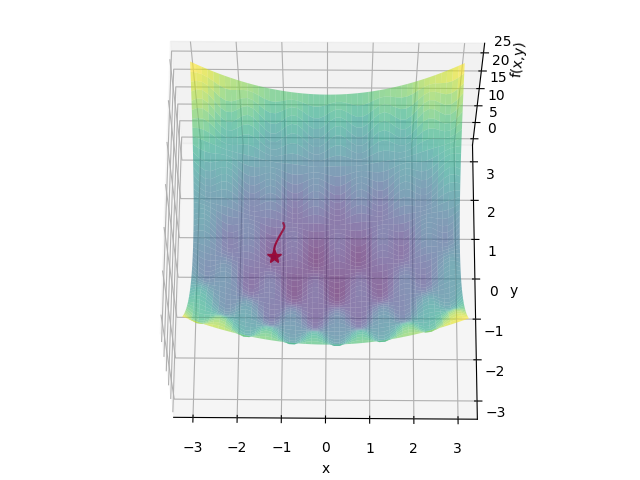
\includegraphics[width=0.6\textwidth]{Figure_2.png}
    \end{figure}
    \begin{figure}[h]
        \caption{Ejecución del algoritmo sobre $f$ con $\eta = 0.1$}
        \centering
        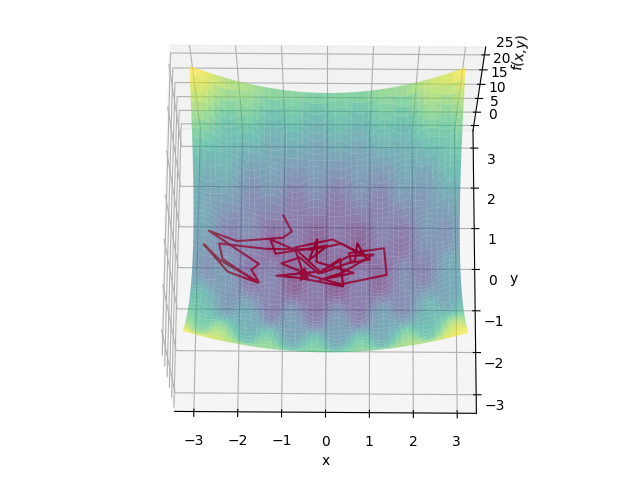
\includegraphics[width=0.6\textwidth]{Figure_3.png}
    \end{figure}
    En la figura 2 podemos ver que el algoritmo ha seguido un recorrido uniforme, encontrando un \textbf{mínimo local}. \par
    Aunque en la figura 3, los pasos se han visto muy dispersos durante la ejecución del algoritmo con resultados peores que
    con una $\eta$ menor, de manera que este valor de $\eta$ no es adecuado para aplicarlo en la ejecución de este algoritmo. \par

    \pagebreak

    En la siguiente tabla podemos ver otros ejemplos de ejecución, cambiando
    el punto inicial $w_0$ con el que se inicia el algoritmo y su tasa de aprendizaje $\eta$ \par
    \begin{figure}[h]
        \begin{center}
            \begin{tabular}{ |c|c|c| }
                \hline
                & $\eta = 0.1$ & $\eta = 0.01$\\
                \hline
                (-0.5,-0.5) & (-1.987, -0.005) = 3.947 & (-0.244, 0.415) = -1.524\\
                \hline
                (1,1) & (0.557, -0.311) = 1.09 & (0.731, 0.414) = -1.037 \\
                \hline
                (2.1,-2.1) & (-1.638, -0.273) = 1.679 & (1.665, -1.173) = 4.634\\
                \hline
                (-3,3) & (0.244, -0.324) = -1.43 & (-2.189, 0.587) = 3.694\\
                \hline
                (-2,2) & (-0.813, 0.491) = 2.986 & (-1.664, 1.171) = 4.634\\
                \hline
            \end{tabular}
        \end{center}
        \caption{Tabla de ejecuciones con distintas $w_0$ y $\eta$}
    \end{figure}
    \section{Conclusión}
    \textbf{¿Cuál es la verdadera dificultad de encontrar el mínimo global de una función arbitraria?} \par
    Podemos ver en la figura 4 que los resultados cambian al usar una $\eta$ distinta en unos casos u otros. Los mejores casos con
    $\eta = 0.01$ son el primero y el segundo, mientras que el resto de casos son mejores con $\eta = 0.1$.
    El mejor caso en general ha sido el primero con $\eta = 0.01$. \emph{¿Por qué?} \par
    Porque el punto inicial era el más próximo al origen de coordenadas y el cual estaba más cerca del supuesto
    mínimo global de la función, ya que ha dado un resultado mejor que el resto. Aunque esto no pasa con
    $\eta = 0.1$ al ser un valor tan elevado que el algoritmo no llega a converger en esa zona. \emph{¿Por qué han conseguido mejores resultados con una $\eta$ más pequeña?} \par
    Porque el punto estaba lo suficientemente cerca del mínimo global que en las siguientes iteraciones podía seguir
    un recorrido prácticamente uniforme y con pasos cada vez más cortos, llegando a converger en un mínimo. Esto también
    puede verse en el segundo caso, pero no en el resto de casos, ya que están suficientemente alejados del origen
    de manera que el valor de $\eta$ no llega a ser suficientemente grande y no llegan a iterar lo suficientemente rápido antes
    de alcanzar el máximo de iteraciones. \par

    \paragraph*{\textbf{En resumen}}La verdadera dificultad de este problema está en acertar con un punto inicial $w_0$ que esté
    lo suficientemente lejos o cerca (según $\eta$) que sea capaz de llegar al mínimo global en un máximo de $N$
    iteraciones que también sea acertada. \par
    Una posible solución sería adaptar $\eta$ de modo que sea directamente
    proporcional a la distancia recorrida, pero el único inconveniente es que también puede converger hacia
    mínimos locales. En mi opinión, podría ser una solución acertada si tenemos conocimiento sobre la función, es decir,
    saber donde podría estar el mínimo global, y en este caso adaptar $\eta$ según la distancia con respecto al mínimo.

    % Con los ejemplos vistos anteriormente, tantos los representados en la tabla como representados en gráficas 3D en el
    % apartado anterior, hemos visto que para la correcta ejecución el algoritmo es necesario \textbf{encontrar una tasa de aprendizaje $\eta$ equilibrada de forma que no cause que el algoritmo \emph{pierda el control} sobre
    % los pasos en cada una de sus iteraciones ni que itere a un ritmo demasiado pequeño, ya que podría no llegar antes de alcanzar las $N$ iteraciones}.\par
    % Y además, este mismo problema \textbf{también puede depender del punto inicial} $w_0$, porque en el primer ejemplo de la tabla
    % se ha llegado a conseguir un mejor resultado con una $\eta$ más pequeña que con $\eta = 0.1$, caso que no sucedía con los tres últimos ejemplos.
    % En conclusión, la dificultad a la hora de aplicar este algoritmo es \textbf{encontrar valores equilibrados para $\eta$ según $w_0$}. \par
    % Se podría dar el caso de que $N$ también influye, pero pueden existir casos en los que itere infinitamente ya que el gradiente tomado pueda
    % ser demasiado grande y que necesite parar obligatoriamente.

    \pagebreak

    \part{Regresión lineal}
    \section{Números manuscritos}
    Siendo las matrices:
    \begin{itemize}
        \item[\textbf{w}:]Los coeficientes del modelo lineal actual
        \begin{equation*}
            \textbf{w} =
            \begin{bmatrix}
                w_0 & w_1 & w_2 \\
            \end{bmatrix}
            \qquad w_i \in \mathbb{R}
        \end{equation*} 
        \item[\textbf{X}:]Los datos de la muestra
        \begin{equation*}
            \textbf{X} =
            \begin{bmatrix}
                x_{10} & x_{11} & x_{12} \\
                x_{20} & x_{21} & x_{22} \\
                \vdots & \vdots & \vdots \\
                x_{N0} & x_{N1} & x_{N2} \\
            \end{bmatrix}
        \end{equation*}
        Los elementos $ x_{i0}$ valen 1
        y el par restante $(x_{i1}, x_{i2}) \in \mathbb{R}$
        representan el nivel medio de gris
        y la simetría de cada número manuscrito $i$
        \item[\textbf{y}:]Los datos objetivo, esto es, los valores que se pretenden alcanzar
        \begin{equation*}
            \textbf{y} = 
            \begin{bmatrix}
                y_0 & y_1 & \dots & y_N \\
            \end{bmatrix}
            \qquad y_i \in \{-1,1\}
        \end{equation*} 
    \end{itemize}
    
    \subsection{Gradiente descendente estocástico}
    El planteamiento del problema es bastante similar al del ejercicio anterior. Esta vez, el objetivo es
    encontrar un modelo de regresión lineal $\textbf{w}$ tal que sea capaz de distinguir unos elementos de otros
    dentro de la muestra \textbf{x} con el mínimo error posible. Al ser una variante estocástica, tendremos la
    muestra dividida en subconjuntos de un tamaño $M$ equitativo, razonable y sin dejar algún dato sin escoger.
    En esto último, el algoritmo se encargará de escoger un valor adecuado, ya que tiene que ser divisor de $N$
    y mucho más pequeño.

    Una posible hipótesis de modelo lineal será el siguiente:
    \begin{equation*}
        h(\textbf{x}_i) = \textbf{w}^\textmd{T}\textbf{x}_i = sign(w_0x_{i0} + w_1x_{i1} + w_2x_{i2})
    \end{equation*}
    Para medir el error entre la hipótesis y el valor objetivo, usaremos la fórmula del error cuadrático medio
    como función a optimizar:
    \begin{equation*}
        E(\textbf{x}_i) = (h(\textbf{x}_i) - y_i)^2
    \end{equation*}
    Por tanto, consideraremos que el error dentro de la muestra $E_{in}$ es:
    \begin{equation*}
        E_{in}(\textbf{w}) = \frac{1}{M}\sum_{i=1}^{M}E(\textbf{x}_i) = (h(\textbf{x}_i) - y_i)^2
    \end{equation*}
    Siendo esta nuestra función a minimizar.

    Este es el auténtico objetivo del algoritmo en este ejercicio, es decir, queremos encontrar una recta que sea capaz
    de dividir unos números de otros \textbf{con el mínimo de errores}

    \pagebreak
    
    Entonces, el gradiente a calcular es:
    \begin{equation*}
        \frac{\partial E_{in}(\textbf{w})}{\partial w_j} =
        \frac{2}{M} \sum_{i=1}^{M}x_{ij}\left( h(\textbf{x}_i) - y_i \right)
    \end{equation*}
    No cambia nada sobre la actualización de la hipótesis, es decir: el punto se sigue actualizando de la
    misma manera
    \begin{equation*}
        w := w - \eta\frac{\partial E_{in}(\textbf{w})}{\partial w}
    \end{equation*}
    Y ahora formalizamos el algoritmo.

    \begin{algorithmic}
        \Function{SGD}{$\textbf{X}$, $\textbf{y}$, $\eta$, $max$\space$iters$}
        %\If{$f$ is not derivable}
        %    \State\Return
        %\EndIf
        \State{$iter \gets 0$}
        \State{$w \gets 0$}
        \State{$data \gets \textbf{X}$}
        \State{$batchsize \gets 2$}
        \While{$(N$ \% $batchsize) \neq 0$ \textbf{and} $batchsize <$ $(N \div 2)$}
            \State{$batchsize \gets batchsize+1$}
        \EndWhile
        \State{$\textit{number of batches} \gets N \div batchsize$}
        \Do
            \State{$data \gets \textnormal{SHUFFLE(\textit{data})}$}
            \State{$minibatches \gets \textnormal{SPLIT(\textit{data}, \textit{number of batches)}}$}
            \For{$minibatch \in minibatches$}
                \State{$iter \gets iter + 1$}
                \State{$w \gets w - \eta \cdot \frac{\partial E_{in}(\textbf{w})}{\partial \textbf{w}}$}
            \EndFor
        \doWhile{$iter \leq max$\space$iters$}
        \State{\Return{$w$}}
        \EndFunction
    \end{algorithmic}
    Denotamos que este algoritmo busca un tamaño de subconjunto: \linebreak
    \begin{center}
        $batchsize \in [2,N \div2 ] \in \mathbb{N}$
        t.q $N$ div $batchsize$
    \end{center}

    Podemos poner un valor minimo del algoritmo más grande, pero puede influir negativamente en las actualizaciones
    de $w$. Al trabajar con el mismo caso, siempre se dará que $batchsize = 7$, de modo que tendremos 227 $batches$.
    Además, por simplicidad, asumiremos que \textit{max iters} = 400.
    \vspace*{0.1in}
    
    \textbf{¿Y si cambiaramos sus valores?}

    El resultado de la ejecución empeoraría con un tamaño de subconjunto más grande, además de su tiempo de ejecución.
    Demostrado experimentalmente.
    \vspace*{0.1in}


    Ejecutando SGD con $\eta = 0.2$, obtenemos los siguientes resultados:
    \begin{center}
        $\textbf{w} \approx \begin{bmatrix}
            -2.514 & -0.271 & -1.080 \\
        \end{bmatrix}$
        \qquad
        \begin{tabular}{ |c|c|c| }
            \hline
            & \textbf{Error} & \textbf{Fallos} \\
            \hline
            \textbf{Training (in)} & 0.128 & 5 \\
            \hline
            \textbf{Test (out)} & 0.094 & 10 \\
            \hline
        \end{tabular}
    \end{center}
    Podemos ver el modelo gráficamente en la figura 5, en la página siguiente.

    Si aumentamos $\eta$ la recta que representa al modelo lineal baja drásticamente, tanto de
    forma que la importancia del valor que posea
    \pagebreak
    \begin{figure}[h]
        \caption{Representación de \textbf{w} y los datos de entrenamiento y de test, respectivamente}
        \centering
        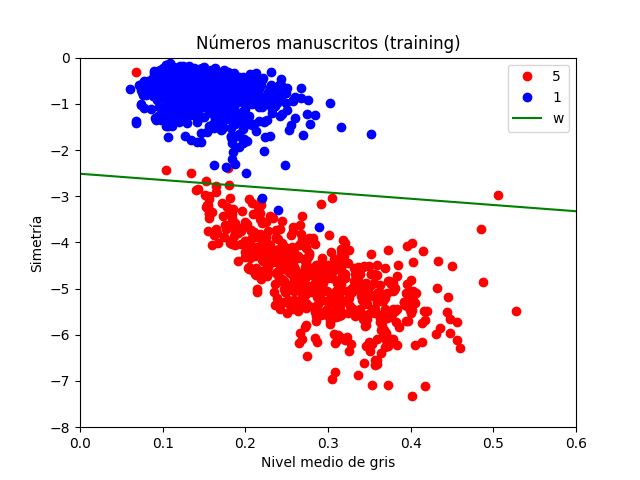
\includegraphics[width=0.65\textwidth]{Figure_4.png}
        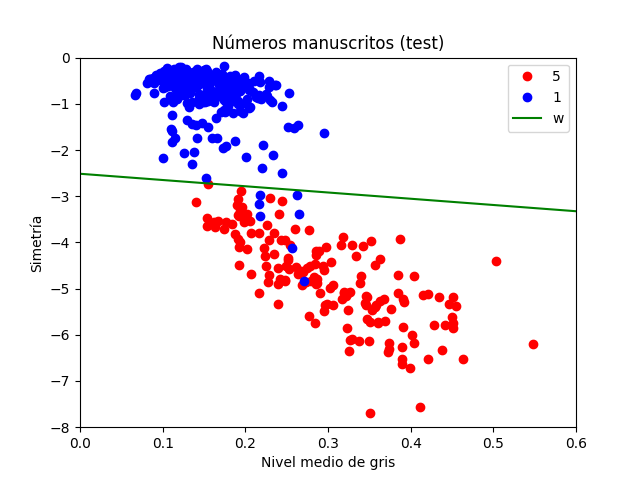
\includegraphics[width=0.65\textwidth]{Figure_5.png}
    \end{figure}





    \pagebreak
    \subsection{Pseudoinversa}
    Este es un método que no necesita iterar, ya que solo se basa en operaciones con matrices.
    Esto es, podemos encontrar un modelo lineal a nuestro problema sin necesidad de iterar
    y sin necesidad de escoger una $\eta$.
    \begin{equation*}
        \textbf{w} = \textbf{X}^\dagger \textbf{y}
    \end{equation*}
    La única complejidad de este método se encuentra en $\textbf{X}^\dagger$, la pseudoinversa de \textbf{X}.

    \begin{equation*}
        \textbf{X}^\dagger = (\textbf{X}^{T}\textbf{X})^{-1}\textbf{X}^T
    \end{equation*}

    Ya que la multiplicación $(\textbf{X}^{T}\textbf{X})^{-1}$ puede llegar a ser inviable
    computacionalmente debido al tamaño que puede llegar a tener \textbf{X} o la forma que tenga la matriz
    de manera que directamente no se pueda realizar la multiplicación, que se da prácticamente casi siempre. \par
    Aplicaremos descomposición en valores singulares, resolviendo el problema de la forma de la matriz:
    \begin{equation*}
        \textbf{X} = \textbf{UDV}^T
    \end{equation*}
    \begin{equation*}
        \textbf{X}^{T}\textbf{X} = \textbf{VDDV}^{T}
    \end{equation*}

    Esto último puede hacerse en Python gracias al método de NumPy: \verb/numpy.linalg.svd()/,
    que devuelve las matrices \textbf{U}, \textbf{D}, y $\textbf{V}^T$
    Es importante realizar la transformación siguiente antes de proceder:
    \begin{center}
        \verb/D = np.diag(d)/
    \end{center}
    Siendo \verb\d\ la segunda matriz devuelta por el método anterior para el SVD.

    \vspace*{0.2in}
    Una vez calculado \textbf{w}, tenemos los siguientes resultados:
    \begin{center}
        $\textbf{w} \approx \begin{bmatrix}
            -1.115 & -1.248 & -0.497 \\
        \end{bmatrix}$
        \qquad
        \begin{tabular}{ |c|c|c| }
            \hline
            & \textbf{Error} & \textbf{Fallos} \\
            \hline
            \textbf{Training (in)} & 0.02 & 8 \\
            \hline
            \textbf{Test (out)} & 0.066 & 7 \\
            \hline
        \end{tabular}
    \end{center}
    \pagebreak
    \begin{figure}[h]
        \caption{Representación de \textbf{w} y los datos de entrenamiento y de test, respectivamente}
        \centering
        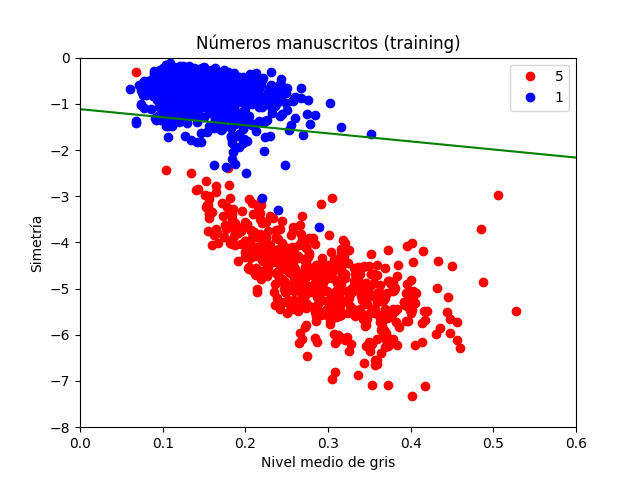
\includegraphics[width=0.65\textwidth]{Figure_8.png}
        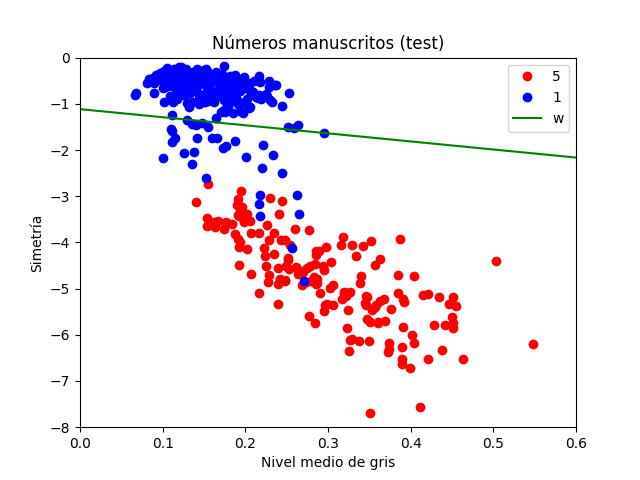
\includegraphics[width=0.65\textwidth]{Figure_9.png}
    \end{figure}

    
    \pagebreak
    \section{Clasificación de datos uniformemente aleatorios}
    \subsection{Modelo lineal}
    Ahora vamos a considerar que \textbf{X} es un conjunto coordenadas de $N = 1000$ puntos
    aleatorios dentro del rango $[-1,1] \times [-1,1]$ y tenemos que clasificarlos con respecto a una
    función $f$
    \begin{equation*}
        f(x_1,x_2) = sign((x_1 - 0.2)^2 + x_2^2 - 0.6) \qquad f:\mathbb{R}^2 \to \{-1,1\}
    \end{equation*}
    De manera que si el punto dado está dentro de la función dará -1, y 1 en caso contrario.
    Es importante decir que existe un 10\% de ruido dentro de cada muestra, es decir, un 10\%
    de los puntos estarán clasificados incorrectamente.
    
    Usaremos SGD para la regresión lineal en este tipo de problemas.
    No obstante, si seguimos aplicando regresión lineal, tendremos los siguientes resultados
    (esta vez no hemos generado un conjunto test).
    \begin{center}
        $\eta = 0.1$
        \qquad
        $\textbf{w} \approx \begin{bmatrix}
            -0.2 & -0.044 & -0.369 \\
        \end{bmatrix}$
        \qquad
        \begin{tabular}{ |c|c|c| }
            \hline
            & \textbf{Error} & \textbf{Fallos} \\
            \hline
            \textbf{Training (in)} & 1.64 & 410 \\
            \hline
        \end{tabular}
    \end{center}
    Podemos ver que son muchos fallos (mas o menos la mitad de la muestra), pero esto se debe
    a que la recta \emph{corta por la mitad} el grupo de puntos dentro de $f$ que necesita separar
    de los de fuera, esto se puede ver en la figura 7. Además, \textbf{el w resultante puede variar}.
    \begin{figure}[h]
        \caption{Representación de \textbf{w} y los $N$ puntos clasificados por $f$}
        \centering
        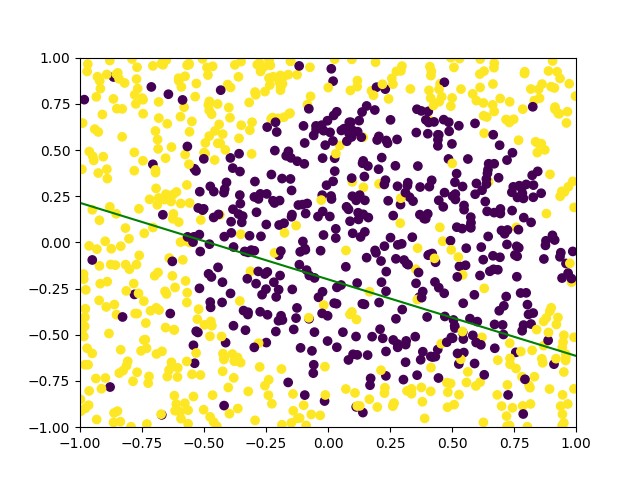
\includegraphics[width=0.5\textwidth]{Figure_6.png}
    \end{figure}

    Ahora vamos a realizar este mismo experimento 1000 veces y vamos a calcular el error medio de todas las muestras
    de entrenamiento y también generaremos una muestra adicional en cada iteración para el test.

    \begin{center}
        \begin{tabular}{ |c|c|c| }
            \hline
            Medias & \textbf{Training} & \textbf{Test} \\
            \hline
            \textbf{Error} & 1.833 & 1.839 \\
            \hline
            \textbf{Fallos (\%)} & 45.972 & 46.272 \\
            \hline
        \end{tabular}
    \end{center}

    \paragraph*{\textbf{Entonces, ¿que podemos hacer para reducir el error?}}Tenemos que transformar el conjunto de características
    y aplicar regresión no linear, esto implica modificar $h(\textbf{x})$ y por tanto \textbf{w} y la longitud de cada
    \textbf{x}

    \pagebreak

    \subsection{Modelo no lineal}
    A cada vector de características \textbf{x} se le aplica una transformación $\phi$ y pasa a ser:
    \begin{equation*}
        (1,x_1,x_2) \to (1,x_1,x_2,x_1x_2,x_1^2,x_2^2)
    \end{equation*}
    De modo que
    \begin{equation*}
        h(\textbf{x}) = sign(w_0 + w_1x_1 + w_2x_2 + w_3x_1x_2 + w_4x_1^2 + w_5x_2^2) \qquad h:\mathbb{R}^2 \to \{-1,1\}
    \end{equation*}

    No cambia nada más, ahora si volvemos a repetir el experimento, los resultados mejoran:
    \begin{center}
        \begin{tabular}{ |c|c|c| }
            \hline
            Medias & \textbf{Training} & \textbf{Test} \\
            \hline
            \textbf{Error} & 0.945 & 0.952 \\
            \hline
            \textbf{Fallos (\%)} & 23.629 & 23.815 \\
            \hline
        \end{tabular}
    \end{center}

    \begin{figure}[h]
        \caption{Representación de \textbf{w} no lineal y los $N$ puntos clasificados por $f$}
        \centering
        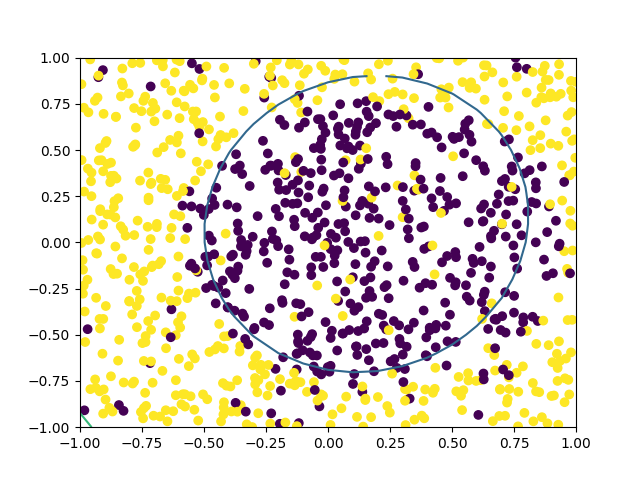
\includegraphics[width=0.5\textwidth]{Figure_7.png}
    \end{figure}

    \subsection{Conclusión}
    \textbf{¿Qué modelo es más adecuado?} \par
    El modelo más adecuado es el no lineal. Podemos ver que los puntos dentro de $f$ componen una forma
    elíptica, de manera que podemos transformar la ecuación lineal a una ecuación de la elipse, como hemos visto
    en esta página con $\phi$. De modo que, en vez de clasificar el punto si está por encima o por debajo de
    la recta, podemos transformar este criterio en ver si el punto está dentro o fuera de la elipse formada por
    nuestro modelo.


\end{document}